\subsection{Neural Networks}

For me, the best way to understand how a neural net works is to look at an actual network and learn by example. One of the classic examples is the XOR function. A discussion of this problem can be found in the Deep Learning book on pg. 167.

Figure \ref{fig:xor} shows what the data looks like for this problem. We have two features, $x_1$ and $x_2$, that can take on two possible values, 0 or 1. We assign another binary variable $y$ to each of the possible combinations of $x_1, x_2$ resulting in $(0,0) = 0, (0,1)=1, (1,1)=1, (1,0)=0$.

The goal here is to find a line that separates the response variable $y$ between its two possible values, 0 or 1. As we can see from the picture this is not possible with the current setup.

 \begin{figure} \label{fig:xor}
\caption{XOR problem}
\centering
 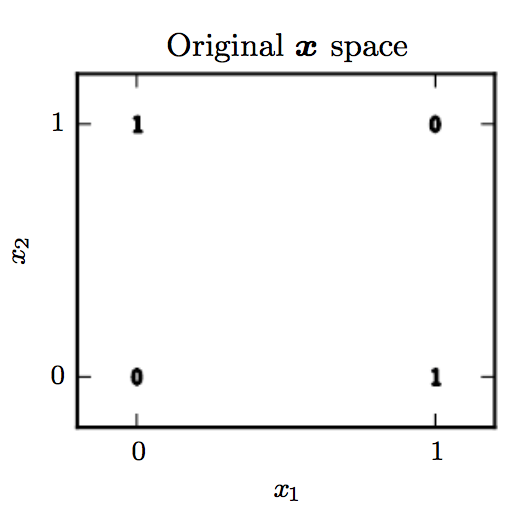
\includegraphics[scale=.7]{xor.png}
 \end{figure}
 
 
 
 \begin{figure} \label{fig:neural_net_image}
\caption{Example of a two layer neural network}
\centering
 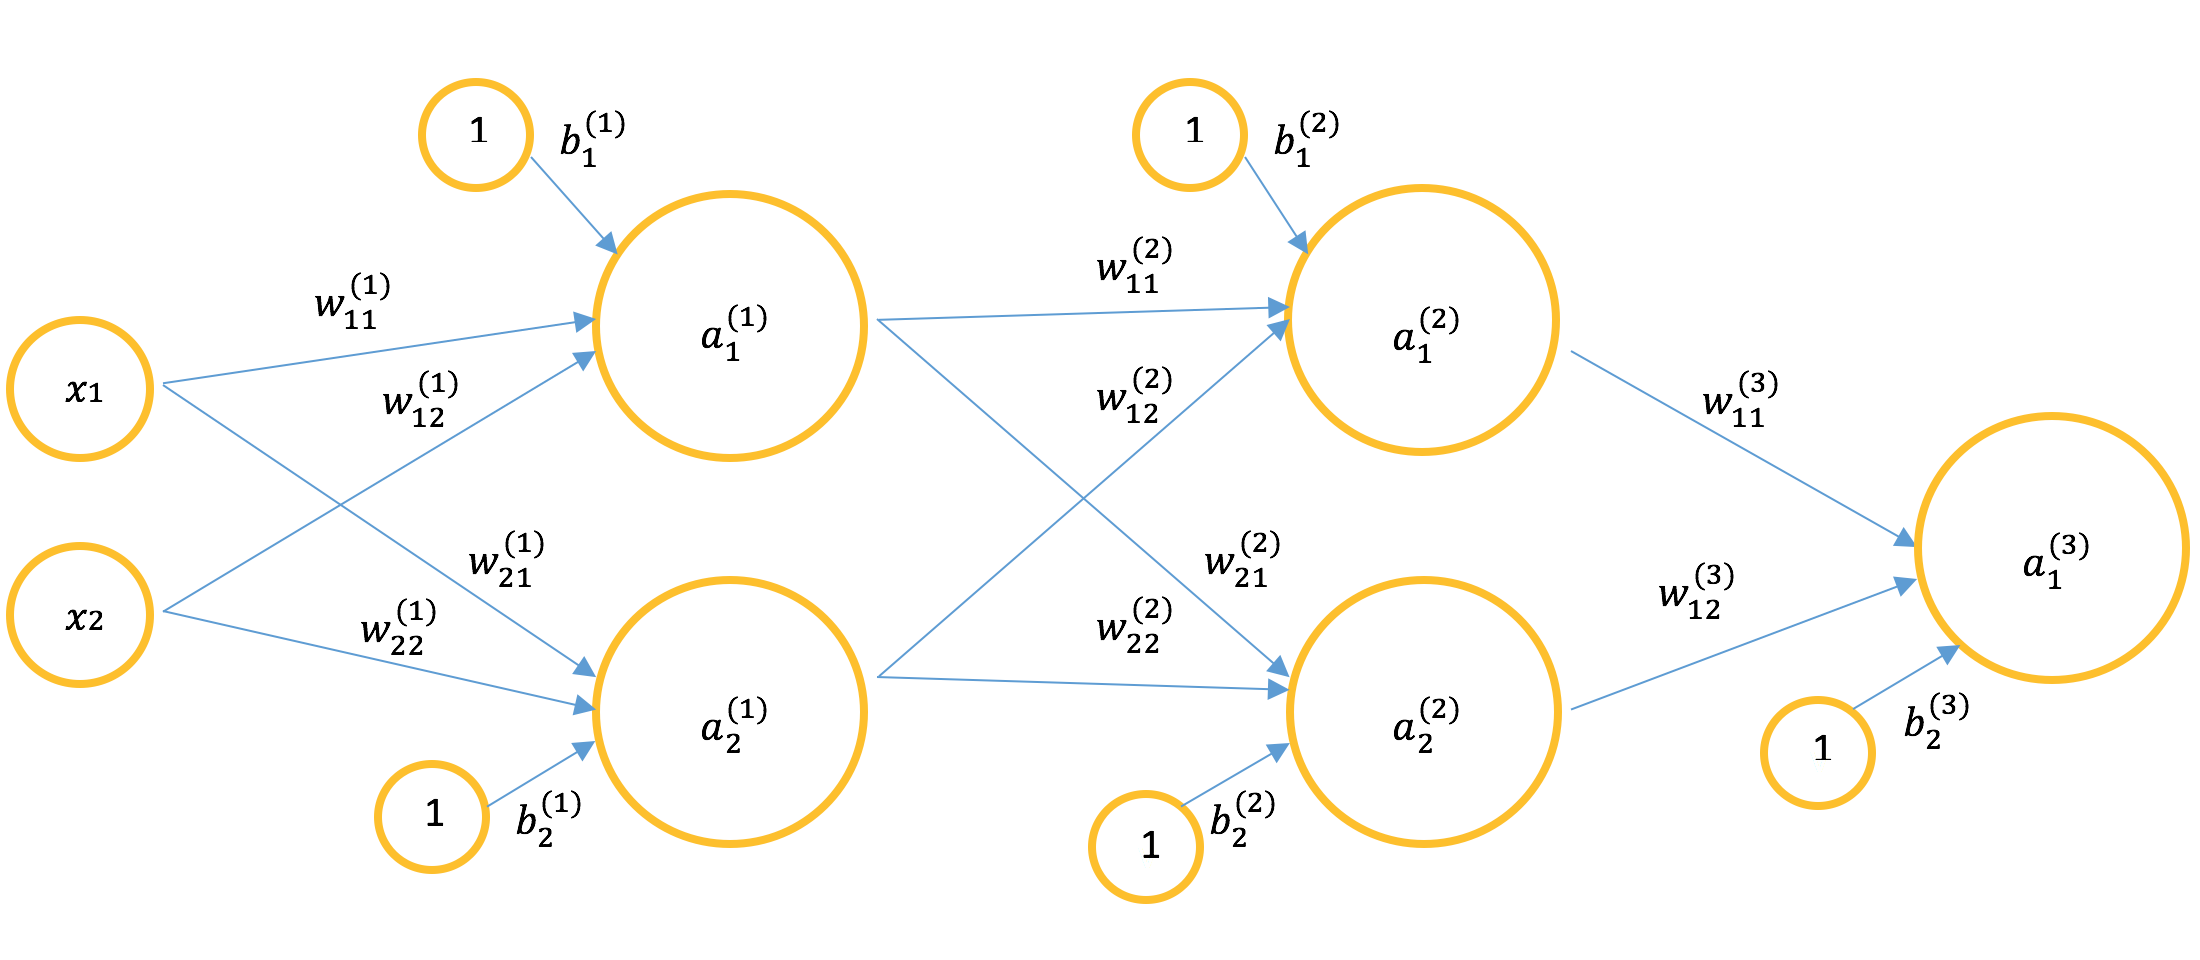
\includegraphics[scale=.3]{neural_net_image.png}
 \end{figure}